\documentclass{book}
\usepackage{graphicx}
\usepackage[english]{babel}
\usepackage{amsthm}
\usepackage{amssymb}
\usepackage{amsfonts}
\usepackage{mdframed}
\usepackage{physics}
\usepackage{tikz}
\usepackage[a4paper, margin=1in]{geometry}
\geometry{a4paper, margin=1in}
\usepackage{xcolor}
\usetikzlibrary{arrows.meta}
\usetikzlibrary{angles,quotes}
\graphicspath{ {./images/} }
\usepackage{svg}
\usepackage{subcaption}
\usepackage{bm}
\usepackage{empheq}
\usepackage{cancel}
\usetikzlibrary{decorations.text}
\usepackage[most]{tcolorbox}
\usepackage{tensor}
\usetikzlibrary{patterns.meta}
%3D
\usepackage{mathtools}
\usepackage{booktabs}
\usepackage{array}
\newcolumntype{C}{>{$}c<{$}}
\usepackage{tikz-3dplot}
\usepackage{appendix}
\usepackage{pgfplots}
\usetikzlibrary{shapes.geometric}
\usetikzlibrary{calc,patterns,angles,quotes}
%Tikz Library
\usetikzlibrary{angles, quotes, intersections}
\usepackage[bb=dsserif]{mathalpha}
\usetikzlibrary{decorations.pathmorphing}

\tikzset{snake it/.style={decorate, decoration=snake}}

\usepackage{etoolbox} % ifthen
\usepackage[outline]{contour} % glow around text
\usetikzlibrary{calc} % for adding up coordinates
\usetikzlibrary{decorations.markings,decorations.pathmorphing}
\usetikzlibrary{angles,quotes} % for pic (angle labels)
\usetikzlibrary{arrows.meta} % for arrow size
\usepackage{xfp} % higher precision (16 digits?)

\usepackage{tcolorbox}

%https://osl.ugr.es/CTAN/macros/latex/contrib/tcolorbox/tcolorbox.pdf
\tcbuselibrary{breakable}
\tcbset{%any default parameters
	width=0.7\textwidth,
	halign=justify,
	center,
	breakable,
	colback=white    
}

\newenvironment{aside}
{\begin{mdframed}[style=0,%
		leftline=false,rightline=false,leftmargin=2em,rightmargin=2em,%
		innerleftmargin=0pt,innerrightmargin=0pt,linewidth=0.75pt,%
		skipabove=7pt,skipbelow=7pt]\small}
	{\end{mdframed}}

\renewcommand{\cleardoublepage}{\clearpage}
\newcommand{\dbar}{\mathrm{d}\hspace*{-0.08em}\bar{}\hspace*{0.1em}}
\title{Statistical Mechanics}
\author{Dominik Szablonski}
\newtheorem{law}{Law}
\newtheorem{klaw}{Law}

\newtcbtheorem{Definitions}{Definition}%
{colback=blue!5!white,colframe=blue!75!black,width=\textwidth,fonttitle=\bfseries}{}

\newtcbtheorem{Theorems}{Theorem}%
{colback=red!5!white,colframe=red!75!black,width=\textwidth,fonttitle=\bfseries}{}

\newtcbtheorem{Postulates}{Postulate}%
{colback=green!5!white,colframe=green!75!black,width=\textwidth,fonttitle=\bfseries}{}

\newtheorem*{theorem}{Theorem}


\setlength\parindent{0pt}
\pgfplotsset{compat=1.18}
\begin{document}
\maketitle

\tableofcontents

\chapter{Basic Thermodynamics}
We will begin by discussing systems with variable particle number. In order to talk as system where the number of particles $N$ varies, we must consider its \textit{chemical potential}, which is defined in terms of the Gibbs free energy,
\begin{equation}
	\mu = \eval{\pdv{G}{N}}_{T,P}.
\end{equation} 
We can find a simpler expression for the chemical potential by considering,
\begin{equation}
	G = G(N,\underbrace{P,T}_{\text{intensive}}).
\end{equation}
We know that the Gibbs free energy is an extensive variable, and so is the number of particles $N$. Thus, we can write,
\begin{equation}
	G = Nf(P,T)
\end{equation}
where $f$ is some function. We actually ind that $f(P,T) = \mu$, so we can write,
\begin{equation}
	\mu = \frac{G}{N}
\end{equation}
from which we can also conclude that $\mu$ is a function of $P$ and $T$. Let us now attempt to generalise this to more than one species of gas. This means that there is more than one extensive variable. For now, let us state without proof,
\begin{equation}
	G = \sum_i \mu_i N_i
\end{equation}
where $N_i$ is the number of particles of a particularly species and $\mu_i$ is its chemical potential. We can then write,
\begin{equation}
	\mu_i = \mu_i\left(T, P, \left\{\frac{N_j}{N}, \forall j \in \mathbb{N}\right\}\right).
\end{equation}
However, if we consider an ideal gas, we can ignore interactions due to other species of gas so we can simply consider, $\mu_i = \mu_i(T, P, N_i/N)$. However,
\begin{align}
	P & = \frac{1}{V}Nk_BT  = \sum_i P_i  & N = \sum_i N_i \\
	& &P_i = \frac{N_i}{V}k_BT \to \text{ Partial pressure} \\
	\implies && \mu_i = \mu_i (T, P_i).
\end{align}
Let us return to considering a single species, and recall,
\begin{align}
	\dd{S} = \frac{1}{T}\dd{E} + \frac{P}{T}\dd{V} && \dd{E} = C_V\dd{T} && V = \frac{Nk_BT}{P}
\end{align}
from which we can show,
\begin{equation}
	- \Delta S = C_P\ln\frac{T}{T_0} - Nk_B\ln\frac{P}{P_0}
\end{equation}
\section{Constant Temperature}
At constant temperature, the Gibbs free energy is,
\begin{align}
	&\Delta G = - T \Delta S = Nk_BT\ln\frac{P}{P_0} \\
	\implies & \Delta \mu = k_BT_0 \ln\frac{P}{P_0}.
\end{align}
\subsection{Chemical Reactions}
If we consider two gasses separated by a membrane, the chemical potential will govern the diffusion of the gasses, and the partial pressures will tend to equalise. Let us consider a reaction between two substances, $A \rightleftharpoons B$. The Gibbs free energy is,
\begin{equation}
	\dd{G} = \mu_A\dd{N}_A + \mu_B \dd{N_B}
\end{equation}
however $\dd{N}_B = \dd{N}_A$, so,
\begin{equation}
	\dd{G} = (\mu_A - \mu_B)\dd{N}_A.
\end{equation}
We have equilibrium when a small change in $N_A$ leaves $G$ unchanged, so $\mu_A = \mu_B$.
\\\\
Let us now consider a reaction with double the reactants and products, $aA + bB \rightleftharpoons xX + yY$, where $a,b,x,y \in \mathbb{Z}$. The number of molecules change by,
\begin{align}
	\dd{N}_B = \frac{b}{a}\dd{N}_A && \dd{N}_X = -\frac{x}{a}\dd{N}_A
\end{align}
Let us write the Gibbs free energy,
\begin{equation}
	\begin{split}
		\dd{G} & = \mu_A\dd{N}_A + \mu_B\dd{N}_B - \mu_X\dd{N}_X - \mu_Y\dd{N}_Y \\ 
		& = \underbrace{\left(\mu_A + \frac{b}{a}\mu_B - \frac{x}{a}\mu_X - \frac{y}{a}\mu_Y\right)}_{0\text{ at equilibrium}}\dd{N}_A \\
		\implies & \mu_A+ b\mu_B = x\mu_X + y\mu_Y
	\end{split}
\end{equation}
We wish to work in terms of moles, so let us write the molar Gibbs free energy,
\begin{equation}
	g^r = xg_X + yg_Y - ag_A - bg_B
\end{equation}
which will be 0 at equilibrium. If we know the $g^r_0 \equiv g_r(T_0, P_0)$ at some reference temperature and partial pressure for all reactants and products, then we can find the molar Gibbs free energy at other partial pressures but the same temperature. Applying our ideal gas assumptions,
\begin{equation}
	\begin{split}
		g_r\left(\left\{P_i\right\},T_0\right) & = g_r(P_0,T_0) + N_Ak_BT_0\left(x\ln\frac{P_X}{P_0} + y\ln\frac{P_Y}{P_0} - a\ln\frac{P_A}{P_0} - b\ln\frac{P_B}{P_0}\right) \\ 
		& = g_r(P_0, T_0) + \ln\left(\left(\frac{P_X}{P_0}\right)^x\left(\frac{P_Y}{P_0}\right)^y\left(\frac{P_0}{P_A}\right)^a\left(\frac{P_0}{P_B}\right)^b\right).
	\end{split}
\end{equation}
At equilibrium $g_r$ = 0, so,
\begin{equation}
	\underbrace{\left(\frac{P_X}{P_0}\right)^x\left(\frac{P_Y}{P_0}\right)^y\left(\frac{P_0}{P_A}\right)^a\left(\frac{P_0}{P_B}\right)^b}_{Q} = \underbrace{\exp\left(-\frac{g_0^r}{RT_0}\right)}_{K_P(T_0)}.
\end{equation}
%and we find,
%\begin{align}
%	Q > K_P && A,B \to X,Y \\
%	Q < K_P && X,Y \to A,B \\
%	Q = 0 && \text{Equilibrium}.
%\end{align}
We can write more generally, an equation for $N$ reactants and $N'$ products,
\begin{equation}
	g_r = \sum_{i=1}^{N'}x_ig_{X_i} - \sum_{j=1}^Na_jg_{A_j}
\end{equation}
and at equilibrium,
\begin{equation}
	\prod_{i=1}^{N'}\left(\frac{P_{X_i}}{P_0}\right)^{x_i}\sum_{j=1}^{N}\left(\frac{P_0}{P_{A_j}}\right) = \exp\left(-\frac{g_0^r}{RT_0}\right)
\end{equation}
\chapter{Statistical Physics}
Before jumping into statistical physics, we must define a few terms,
\begin{Definitions}{Macrostate}{}
	State of a sufficiently large system in equilibrium specified by a few measurable quantities, i.e., $P$, $T$, etc.
\end{Definitions}
\begin{Definitions}{Microstate}{}
	A description of a system consisting of the position and momentum (or quantum states) of every molecule present in the system.
\end{Definitions}
We wish to relate the macrostate to the microstate and predict macroscopic properties from first principles. For each macrostate, there exist many microstates. In order to formulate statistical mechanics, we must assume that a system can access al available microstates, so we can average over al microstates to predict the macrostate.
\section{Microcanonical Ensemble}
\begin{Definitions}{Ensemble}{}
	Collection of objects, which are copies of the system at each point in time. 
\end{Definitions}
We use the ensemble to avoid taking time averages. The ensemble average is given by,
\begin{equation}
	\left<x\right> = \sum_i P_iX_i
\end{equation}
where $P_i$ is the probability of the $i$th microstate, and $X_i$ is the value of $X$ in the $i$th microstate. Let us now say that we have $\nu$ objects in the ensemble, with $\nu_i$ objects in the $i$th microstate, and we denote each object in the ensemble with $\lambda$, we can write,
\begin{equation}
	\left<x\right>  = \frac{1}{\nu} \sum_{\lambda}X_{\lambda} = \frac{1}{\nu}\sum_i\nu_iX_i = \sum_i P_iX_i
\end{equation}
from which we find,
\begin{equation}
	P_i = \frac{\nu_i}{\nu}.
\end{equation}
However, for a system in isolation, we can postulate the following,
\begin{Postulates}{Postulate of Equal a priori Probabilities}{}
	All microstates are equally likely.
\end{Postulates}
Thus, if our total number of microstates is $\Omega$, the probability of the $i$th microstate is,
\begin{equation}
	P_i = \frac{1}{\Omega},\hspace{1em}\forall i.
\end{equation}
\begin{aside}
	For a system with $N$ particles which each can be in one of two states, such that there are $n$ and $N-n$ states respectively, then the total number of microstates is given by,
	\begin{equation}
		\frac{N!}{n!(N-n)!} = {^nC_N}.
	\end{equation}
\end{aside}
\section{Statistical Basis of Entropy}
The number of microstates $\Omega$ for a number of particles $N$ in the system and a set of particles of size $n$ in one state, $m$ in a second state, etc., is given by,
\begin{equation}
	\Omega(n) = \frac{N!}{n!m!\cdots!}.
\end{equation}
For a system with just $N$ total particles and two sets of particles of size $n$, $N-n$ this is,
\begin{equation}
	\Omega(n) = \frac{N!}{n!(N-n)!}.
\end{equation}
For large systems, $\Omega$ rises dramatically. For two possible states, we can write the distribution of microstates as a binomial distribution,
\begin{align}
	\overline{n} = \frac{N}{2} && \sigma_n = \frac{\sqrt{N}}{2} && \frac{\sigma_n}{N} \approx \frac{1}{\sqrt{N}}.
\end{align}
For large $N$, we find that the ensemble average $\left<X\right>$ is entirely dominated by microstates with the most probable $X_i$, denoted $X_{\text{Prob}}$. Thus,
\begin{equation}
	\langle X \rangle = \sum_i P_i X_i \approxeq X_{\text{Prob}}
\end{equation}
which is true within a few $\sigma$ of the most probable value.
\\\\
As the microstate changes, the vast majority of new states have similar (or essential equal) $X_i \approx X_{\text{Prob}}$ so nothing changes at equilibrium.
\\\\
If our system begins out of equilibrium, i.e., $n < N/2$, the time evolution must in principle increase or decrease $n$, but there are vastly more states with greater $n$ and so evolution is overwhelmingly likely to lead to $n \uparrow$ until $n \approx N/2$. 
\\\\
Furthermore, for large $N$, $\Omega(n)$ tends to an exponential,
\begin{equation}
	\Omega(n) = \exp\left(\frac{\left(n - \frac{N}{2}\right)^2}{\frac{N}{2}}\right)
\end{equation}
with mean $N/2$, $\sigma = \sqrt{N}/2$.
\\\\
We might then think that $\Omega \propto S$, but this is not the case. This is because entropy is extensive, whereas we combine microstates by multiplying them together. Instead, the following relation holds,
\begin{equation}
	S = k_B \ln\Omega.
\end{equation}
\section{Spin-Half Paramagnet}
An atom or molecule of a spin-$\frac{1}{2}$ paramagnet has $s = \frac{1}{2}$, $\abs{\vb{S}} = \frac{\sqrt{3}}{2}\hbar$, $S_z = \pm \frac{1}{2}\hbar$. Each molecule has a magnetic moment $\vb*{\mu}$ such that $\mu_z = \pm \mu$. The total magnetisation of the sample is then given by,
\begin{equation}
	\begin{split}
		m & = n_{\uparrow} + n_{\downarrow}(-\mu) \hspace{2em} n_{\downarrow} = N - n_{\uparrow} \\
		& = (2n_{\uparrow} - N)\mu	\end{split}
\end{equation}
If there is a magnetic field, the energy is given by,
\begin{equation}
	 U = -\vb{m}\cdot\vb{B}
\end{equation}
with each atom having energy $\mp \mu B$ for spin $\updownarrow$, as the atoms align to lower energy. The total energy is then,
\begin{equation}
	U = n_{\uparrow}(-\mu B) + n_{\downarrow}(\mu B) = (N - 2n_{\uparrow})\mu B = mB.
\end{equation}
The microstates are then specified by specifying the spin of each atom. For $N$ atoms there are $2^N$ microstates. If there is no external magnetic field, the atoms have equal probability of being $\uparrow$ or $\downarrow$, thus equilibrium will be reached at $m=0$.
\subsection{Energy to Temperature}
\begin{figure}
	\centering
	\begin{tikzpicture}
		\draw (0,0) rectangle (4,4);
		\fill[pattern={Lines[angle=45,distance=0.5cm]}] (0,4) rectangle (4,4.25);
		\fill[pattern={Lines[angle=45,distance=0.5cm]}] (0,0) rectangle (-0.25,4);
		\fill[pattern={Lines[angle=45,distance=0.5cm]}] (0,0) rectangle (4,-0.25);
		\fill[pattern={Lines[angle=45,distance=0.5cm]}] (4,4) rectangle (4.25,0);
		\draw[dashed] (2,0.1) -- (2,3.9);
		\draw (1.9,0.1) -- (2.1,0.1);
		\draw (1.9,3.9) -- (2.1,3.9);
		\node at (1,3) {$E_1$};
		\node at (1,2) {$N_1$};
		\node at (1,1) {$V_1$};
		\node at (3,3) {$E_2$};
		\node at (3,2) {$N_2$};
		\node at (3,1) {$V_2$};
	\end{tikzpicture}
	\caption{}
	\label{fig:isolated}
\end{figure}
Let us consider an isolated system separated by a permeable membrane, as in figure \ref{fig:isolated}, such that,
\begin{align}
	E_1 + E_2 = E && N_1 + N_2 = N && V_1 + V_2 = V
\end{align}
are fixed. We further have,
\begin{align}
	\Omega = \Omega_1 + \Omega_2 && S = k_B\ln\Omega_1 + k_B\ln\Omega_2 = S_1 + S_2.
\end{align}
Let us consider the heat flow in the system only, keeping $V_1,V_2$ and $N_1,N_2$ constant. We have,
\begin{equation}
	\dd{S} = \left(\pdv{S_1}{E_1}\right)_{V_1,N_1}\dd{E_1} + \left(\pdv{S_2}{E_2}\right)_{V_2,N_2}\dd{E_2}
\end{equation}
however, $\dd{E}_1 = - \dd{E}_2$, so,
\begin{equation}
	\dd{S} = \left(\left(\pdv{S_1}{E_1}\right)_{V_1,N_1} - \left(\pdv{S_2}{E_2}\right)\right)\dd{E}_1
\end{equation}
and equilibrium is reached when,
\begin{equation}
	\left(\pdv{S_1}{E_1}\right)_{V_1,N_1} = \left(\pdv{S_2}{E_2}\right)_{V_2,N_2}
\end{equation}
this equation thus governs heat transfer. If $\dd{E} > 0$, then $\dd{S} >0$ and,
\begin{equation}
	\left(\pdv{S_1}{E_1}\right)_{V_1,N_1} > \left(\pdv{S_2}{E_2}\right)_{V_2,N_2}
\end{equation}
so heat flows from high $\left(\pdv{S}{E}\right)_{V,N}$  to low $\left(\pdv{S}{E}\right)_{V,N}$, so we require $T$ to decrease with $\left(\pdv{S}{E}\right)_{V,N}$. Furthermore, $\left(\pdv{S}{E}\right)_{V,N} > 0$ for almost al systems, so an appropriate guess would be to say,
\begin{equation}
	\left(\pdv{S}{E}\right)_{V,N} = \frac{1}{T}. \label{eq:1/T}
\end{equation}
Repeating similar process, but only allowing $V_1, V_2$ to vary, we find that $\left(\pdv{S}{V}\right)_{E,N}$ governs how the partition moves. If $\left(\pdv{S_1}{V_1}\right)_{E_1,N_1} > \left(\pdv{S_2}{V_2}\right)_{E_2,N_2}$, we have that $V_1$ increases and $V_2$ decreases, like pressure. Thus, we can link this to classical thermodynamics,
\begin{equation}
	\left(\pdv{S}{V}\right)_{E,N} = \frac{P}{T}.
\end{equation}
Considering variable particle number, we obtain,
\begin{equation}
	\left(\pdv{S}{N}\right)_{V,E} = \frac{\mu}{T}
\end{equation}
and thus, we can obtain the fundamental thermodynamic relation,
\begin{equation}
	\dd{S} = \frac{1}{T}\dd{E} + \frac{P}{T}\dd{V} - \frac{\mu}{T}\dd{N}.
	\end{equation}
\subsection{Isolated spin-$\frac{1}{2}$ paramagnet in the presence of a magnetic field}
Let us return to the ideal paramagnet. The total energy is given by,
\begin{equation}
	E = \mu B \left(N - 2n_{\uparrow}\right) = \mu B \left(2n_{\downarrow} - N\right).
\end{equation}
The reversible work done is,
\begin{equation}
	\dbar W^{\text{rev}} = -m\dd{B} \implies \frac{m}{T} = \left(\pdv{S}{B}\right)_{E,N}.
\end{equation}
The entropy of the paramagnet is,
\begin{equation}
	\begin{split}
	S & = k_B \ln \Omega(E, B) \\
	& = k_B ln\left(\frac{N!}{n_{\uparrow}!\left(N - n_{\uparrow}\right)!}\right).
	\end{split}
\end{equation}
where $\Omega$ is a function of $E,B$ as $n_{\uparrow}$ and $E$ co-vary as,
\begin{equation}
	n_{\uparrow} = \frac{1}{2}\left(N - \frac{E}{\mu B}\right).
\end{equation}
We will use Stirling approximation,
\begin{equation}
	\ln (x!) = x\ln x - x \label{eq:stiring}
\end{equation}
which holds for large $x$. By writing out,
\begin{equation}
	S = k_B \left[\ln(N!) - \ln(n_{\uparrow}!) - \ln \left((N-n_{\uparrow})!\right)\right]
\end{equation}
and using equation \eqref{eq:stiring},
\begin{equation}
	S = k_B\left[N\ln(N) - n_{\uparrow}\ln(n_{\uparrow}) - (N-n)\ln(N-n)\right]
\end{equation}
While in equilibrium, $n_{\uparrow} = n_{\downarrow} = \frac{N}{2}$, in which case,
\begin{equation}
	S = k_B\ln(2^N)
\end{equation}
which indicates that essentially all microstates are at equilibrium. Applying the chain rule to equation \eqref{eq:1/T}, we find,
\begin{equation}
	\frac{1}{T} = \left(\pdv{S}{n_{\uparrow}}\right)_{N}\left(\pdv{n_{\uparrow}}{E}\right)_B.
\end{equation}
We then find,
\begin{equation}
	\left(\pdv{S}{n_{\uparrow}}\right)_B = k_B \ln \frac{N - n_{\uparrow}}{n_{\uparrow}}
\end{equation}
and,
\begin{equation}
	\left(\pdv{n_{\uparrow}}{E}\right)_B = -\frac{1}{2\mu B}
\end{equation}
thus,
\begin{equation}
	\frac{1}{T} = \frac{k_B}{2\mu B}\ln \left(\frac{n_{\downarrow}}{n_{\uparrow}}\right).
\end{equation}
For the magnetic field,
\begin{equation}
	\frac{m}{T} = \left(\pdv{S}{B}\right)_{E,N} = \frac{k_BE}{2\mu B^2}\ln \left(\frac{n_{\downarrow}}{n_{\uparrow}}\right) \implies m = -\frac{E}{B}.
\end{equation}
For a varied magnetic field, we can write the ratio of spin-down to spin up electrons as,
\begin{equation}
	\frac{n_{\downarrow}}{n_{\uparrow}} = \exp\left(-\dfrac{2\mu B}{k_B T}\right). \label{eq:ratio}
\end{equation}
\section{The Ideal Gas}
We can derive the equation for a classical, ideal gas. Let us consider a volume divided into small cells, such that we can treat position microstates as discrete, of volume $\Delta V$. There are $V/\Delta V$ cells, and $\left(V/\Delta V\right)^N$ microstates. Thus, the entropy is,
\begin{equation}
	S = N k_B \ln\frac{V}{\Delta V}.
\end{equation}
We then find,
\begin{equation}
	\begin{split}
		\frac{P}{T} & = \left(\pdv{S}{V}\right)_{E,N} = Nk_B\frac{1}{V} \\
		& \implies PV = Nk_BT.
	\end{split}
\end{equation}
\chapter{Statistical Physics of Non-Isolated Systems}
In order to find the physics of non-isolated systems, we must fix $T$ and $E$. $\langle E \rangle$ depends on $T$, although there will be microscopic fluctuations. These fluctuations are of an order,
\begin{equation}
	\frac{\Delta E}{\langle E \rangle} \sim \frac{1}{\sqrt{N}}.
\end{equation}
\section{Boltzmann Distribution}
	\begin{figure}
		\centering
		\begin{tikzpicture}
			\draw (0,0) rectangle (4,4);
			\fill[pattern={Lines[angle=45,distance=0.5cm]}] (0,4) rectangle (4,4.25);
			\fill[pattern={Lines[angle=45,distance=0.5cm]}] (0,0) rectangle (-0.25,4);
			\fill[pattern={Lines[angle=45,distance=0.5cm]}] (0,0) rectangle (4,-0.25);
			\fill[pattern={Lines[angle=45,distance=0.5cm]}] (4,4) rectangle (4.25,0);
			\draw (3,0) -- (3,1) -- (4,1);
			\node at (1.5, 2.5) {$R$};
			\node at (1.5, 2) {$E_R$};
			\node at (3.5, 0.75) {$S$};
			\node at (3.5, 0.25) {$\varepsilon$};
		\end{tikzpicture}
		\caption{Isolated system consisting of large reservoir $R$ and small system $S$ such that $S << R$.}
		\label{fig:isolated2}
	\end{figure}
Consider an isolated system as in figure \ref{fig:isolated2}. The total energy of this system is fixed, such that $E = E_R + \varepsilon$. We wish to know, for the $i$th microstate of $S$, what is the probability $p_i$ of finding it in that microstate, with an associated energy $\varepsilon_i$. This probability is directly proportional to the total number of microstates,
\begin{equation}
	\begin{split}
		p_i & \propto \Omega_{S+R} = \Omega_S\Omega_R \\
		& \propto \Omega_R(E - \varepsilon_i) = e^{\frac{1}{k_BT}S_R(E - \varepsilon_i)}.
	\end{split}
\end{equation}
Given $E << \varepsilon_i$, we can perform a taylor expansion up to the first order,
\begin{equation}
	S_R(E - \varepsilon_i) = S_R(E) - \varepsilon_i\underbrace{\eval{\pdv{S_R}{E}}_{E_R = E}}_{\frac{1}{T}}.
\end{equation}
Thus, we have,
\begin{equation}
	p_i \propto e^{\frac{1}{k_B}S_R(E)}e^{-\frac{\varepsilon_i}{k_BT}}
\end{equation}
which we can write as,
\begin{align}
	p_i= \frac{1}{Z}e^{-\frac{\varepsilon_i}{k_BT}} && Z = \sum_je^{-\frac{\varepsilon_j}{k_BT}} \label{eq:Z}
\end{align}
which is the Boltzmann distribution, with normalisation $Z$.
\subsection{Paramagnet}
Let us consider a paramagnet consisting of a single atom. There are 2 states, $\uparrow E = -\mu B$ and $\downarrow E = \mu B$. Therefore, the normalisation is,
\begin{equation}
	Z = e^{\frac{\mu B}{k_BT}} + e^{-\frac{\mu_B}{k_BT}}
\end{equation}
and the probability of spin up and spin down are,
\begin{align}
	P(\uparrow) = \frac{e^{\frac{\mu B}{k_B T}}}{Z} && P(\uparrow) = \frac{-e^{\frac{\mu B}{k_B T}}}{Z}
\end{align}
whose ratio is,
\begin{equation}
	\frac{P(\downarrow)}{P(\uparrow)} = e^{-\frac{2\mu B}{k_BT}}
\end{equation}
which is identical to eq. \eqref{eq:ratio}.
\section{Partition Function}
The normalisation factor $Z$ in equation eq. \eqref{eq:Z} is also known as the \textit{partition function}. It is useful to us, as we are able to extract useful information about different macroscopic properties of a system. If we define $\beta = 1/k_BT$, we have,
\begin{align}
	\langle E \rangle & = \frac{\sum_i\varepsilon_ie^{\varepsilon_i\beta}}{\sum_j e^{-\varepsilon_j \beta}} = -\pdv{\ln(Z)}{\beta} \\
	\langle C_V \rangle & = \pdv{\langle E \rangle}{T} = -\frac{1}{k_BT^2}\pdv[2]{\ln(Z)}{\beta} \\
	\langle E^2 \rangle & = \frac{1}{Z}\pdv[2]{Z}{\beta}\\
	\Delta E^2 & = \left(k_B T\right)^2 \frac{C_V}{k_B}.
\end{align}
\section{Helmholtz Free Energy and Entropy}
We wish to consider a system larger than $S$. Let us consider $\nu$ copies of the system, all in thermal contact. This can be considered a canonical ensemble because, together, they are large enough to have a well defined $T$. Then, for any individual $S$, the rest of the system is the reservoir, whose probabilities follow the Boltzmann distribution.
\\\\
The ensemble has $\nu_i$ copies in the $i$th microstate, with $p_i = \nu_i/\nu$. The total number of microstates is,
\begin{equation}
	\Omega_{\nu} = \frac{\nu!}{\nu_1!\nu_2!\nu_3!\ldots},
\end{equation} 
and by Stirling's approximation,
\begin{equation}
	\begin{split}
	\ln\Omega_{\nu} &= \nu\ln\nu - \nu -\biggl(\sum_i \nu_i\ln\nu_i - \underbrace{\sum_j\nu_j}_{\nu}\biggr) \\
	& = \nu\ln\nu - \sum_i\nu_i\ln\nu_i \\ & = \sum_i\nu_i(\ln\nu - \ln\nu_i) \\
	& = \sum_i \nu_i\ln\frac{\nu}{\nu_i} \\
	& = -\sum_i\nu_i\ln p_i \\
	& = -\nu\sum_i p_i\ln p_i
	\end{split}
\end{equation}
and by extensivity,
\begin{equation}
	\begin{split}
		\langle S \rangle &= \frac{1}{\nu}\langle S_{\nu}\rangle \\
		& \boxed {= - k_B\sum_ip_i\ln p_i}
	\end{split}
\end{equation}
which is known as the \textit{Gibbs entropy}. Let us check if this works for the macrocanonical ensemble, i.e., $p_i = \frac{1}{\Omega}$. We have,
\begin{equation}
	\begin{split}
	\langle S \rangle &= k_B\sum_i^{\Omega}\frac{1}{\Omega}\ln \Omega \\
	& = k_B \Omega
	\end{split}
\end{equation}
which is what we expect. Furthermore, the Gibbs expression is more general and can be applied to any probability distribution. Let us now apply this to the canonical ensemble, with $p_i = e^{-\varepsilon_i\beta}/Z$,
\begin{equation}
	\begin{split}
	\langle S \rangle &= -k_B\sum_ip_i\left[\ln\left(e^{-\varepsilon_i\beta}\right)-\ln Z\right]\\
	& = -k_B \sum_ip_i\left(\varepsilon_i\beta - \ln Z\right) \\
	& = k_B \left(\frac{1}{k_B T}\langle E \rangle - \ln Z \right) \\
	& = -k_B\frac{1}{k_BT} \pdv{\ln Z}{\beta} + \ln Z
\end{split}
\end{equation}
so we can find $\langle S \rangle$ from $Z$. However, we can rewrite this as,
\begin{equation}
	-k_BT \ln Z = \langle E \rangle + T \langle S \rangle = \langle F \rangle 
\end{equation}
so we find that $Z$ directly gives us $F(T,V)$ or $F(T,B)$, or the Helmholtz free energy. The Helmholtz free energy is the natural potential for a system at fixed energy. Let us then recall the Maxwell relations,
\begin{align}
	S = -\left(\pdv{F}{T}\right)_{V (\text{or } B), N} && P = -\left(\pdv{F}{V}\right)_{T, N} && \mu = \left(\pdv{F}{N}\right)_{V, T}
\end{align}
\subsection{The paramagnet at fixed temperature}
\begin{figure}
	\centering
	\begin{subfigure}{0.45\textwidth}
		\centering
		\begin{tikzpicture}[scale=0.8]
			\begin{axis}[
				xlabel=$\beta$, 
				ylabel =$\langle E \rangle$, 
				domain=0:10,
				ymax=0.1,
				axis y line = left,
				axis x line = middle,
				ticks = none]
				\addplot[blue, samples=100] {-tanh(0.5*x)};
			\end{axis}
			\node at (-0.8,0.1) {$-N\mu B$};
		\end{tikzpicture}
		\caption{$\langle E \rangle$ vs. $\beta$.}
	\end{subfigure}
	\begin{subfigure}{0.45\textwidth}
		\centering
		\begin{tikzpicture}[scale=0.8]
			\begin{axis}[
				xlabel=$T$, 
				ylabel =$\langle E \rangle$, 
				domain=0:10,
				axis y line = left,
				axis x line = middle,
				ymax=0.1,
				ticks = none]
				\addplot[blue, samples=100] {-tanh(1.5/x)};
			\end{axis}
			\node at (-0.8,0.1) {$-N\mu B$};
		\end{tikzpicture}
		\caption{$\langle E \rangle$ vs. $1/T$.}
	\end{subfigure}
	\caption{Function of average energy against $\beta$ and $1/T$.}
	\label{fig:B}
\end{figure}
We had first considered a paramagnet consisting of a single atom, with a single spin, whose partition function is,
\begin{equation}
	Z_1 = e^{\mu B \beta} + e^{-\mu B \beta} = 2\cosh(\mu B \beta)
\end{equation}
and average energy,
\begin{equation}
	\left<E_1\right> = -\mu B \frac{2\sinh(\mu B \beta)}{2\cosh(\mu B \beta)} = -\mu B \tanh(\mu B \beta).
\end{equation}
We can see how this energy varies in figure \ref{fig:B}. We can also look at the heat capacity of the paramagnet,
\begin{equation}
	C_V = \left(pdv{E}{T}\right)_{N,B} = Nk_b(\mu B \beta)^2\sech[2](\mu B \beta)
\end{equation}
which we visualise in figure \ref{fig:cv}.
\begin{figure}
	\centering
	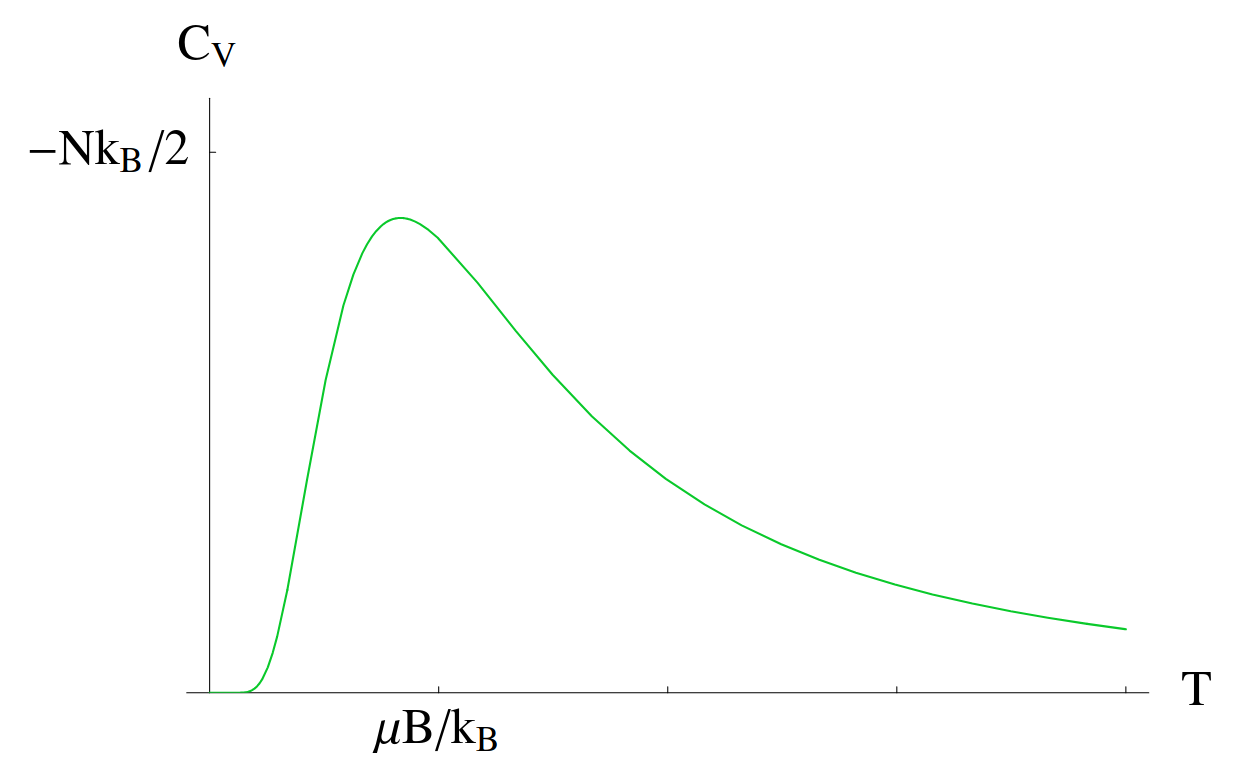
\includegraphics[width=0.45\textwidth]{cv.png}
	\caption{}
	\label{fig:cv}
\end{figure}
\\\\
For $N$ non-interacting spins, we can see that the energy will be $\langle E \rangle = N \langle \varepsilon_1 \rangle$. However, this does not hold for entropy. In order to progress to a paramagnet with $N$ spins, we require the partition function of the entire system, let us call this $Z_N$. This is given by,
\begin{equation}
	Z_N = (Z_1)^N.
\end{equation}
So,
\begin{equation}
	Z_N = \left(e^{\mu B \beta} + e^{-\mu B \beta}\right)^N
\end{equation}
and the Helmholtz free energy is,
\begin{equation}
	F = -Nk_BT\ln(Z_1)
\end{equation}
the entropy is,
\begin{equation}
	\langle S \rangle = N k_B \left(\ln(2\cos(\mu B \beta)) -\mu B \beta \tanh (\mu B \beta)\right)
\end{equation}
and the average magnetic dipole is,
\begin{equation}
	\left<m \right> = -\left<E\right>B.
\end{equation}
\end{document}
